\documentclass[a4paper]{article}
\usepackage[utf8]{inputenc}
\usepackage[spanish, es-tabla]{babel}

\usepackage{amsmath}
\usepackage{amsfonts}
\usepackage{amssymb}

\usepackage{float}
\usepackage{graphicx}
\graphicspath{ {./Imagenes/} }

\usepackage{fancyhdr}

\usepackage{units} 

\pagestyle{fancy}
\fancyhf{}
\lhead{93.54 Métodos Numéricos}
\rhead{Fontecha, Lambertucci, Pouthier, Londero B.}
\rfoot{Página \thepage}



\begin{document}

%%%%%%%%%%%%%%%%%%%%%%%%%%%%%%%%%%%%%%%%%%%%%%%%%%%%%%%%%%%%%%%%%%%%%%%%% 
%								CARATULA								%
%%%%%%%%%%%%%%%%%%%%%%%%%%%%%%%%%%%%%%%%%%%%%%%%%%%%%%%%%%%%%%%%%%%%%%%%% 

\begin{titlepage}
\newcommand{\HRule}{\rule{\linewidth}{0.5mm}}
\center
\mbox{\textsc{\LARGE \bfseries {Instituto Tecnológico de Buenos Aires}}}\\[1.5cm]
\textsc{\Large 93.54 Métodos Numéricos}\\[0.5cm]


\HRule \\[0.6cm]
{ \Huge \bfseries Trabajo práctico N$^{\circ}$2}\\[0.4cm] 
\HRule \\[1.5cm]


{\large

\emph{Grupo 3}\\
\vspace{3px}

\begin{tabular}{lr} 	
\textsc{Fontecha}, María Eugenia  & 58138 \\
\textsc{Lambertucci}, Guido Enrique  & 58009 \\
\textsc{Pouthier}, Florian  & 61337 \\
\textsc{Londero Bonaparte}, Tomás Guillermo  & 58150 \\
\end{tabular}

\vspace{20px}

\emph{Profesor}\\
\vspace{3px}
\textsc{Fierens}, Pablo Ignacio\\ 	
\textsc{Álvarez}, Adrián Omar\\ 

\vspace{100px}

\begin{tabular}{ll}

Presentado: & 02/06/19\\

\end{tabular}

}

\vfill

\end{titlepage}


%%%%%%%%%%%%%%%%%%%%%%%%%%%%%%%%%%%%%%%%%%%%%%%%%%%%%%%%%%%%%%%%%%%%%%%%% 
%								INFORME									%
%%%%%%%%%%%%%%%%%%%%%%%%%%%%%%%%%%%%%%%%%%%%%%%%%%%%%%%%%%%%%%%%%%%%%%%%%


\section{Introducción}

El trabajo presentado consiste en aproximar funciones dadas en ecuaciones diferenciales, mediante el uso del método de Heun o tambien conocido como Runge-Kutta de segundo orden. Estas ecuaciones representan un modelo de crecimiento óseo basado en un balance entre osteoblastos y osteoclastos, obtenidas delel artículo de \textit{Lemaire et al}\footnote{Vincent Lemaire, Frank L. Tobin, Larry D. Greller, Carolyn R. Cho, and
Larry J. Suva. Modeling the interactions between osteoblast and osteoclast
activities in bone remodeling. 229:293–309, 2004.}.

El sistema a aproximar es el siguiente:

\begin{equation}
\frac{dR}{dt} \ = \ D_R \cdot {\pi}_{C} \ - \ \frac{D_B}{{\pi}_{C}} \ \ {I}_{R},
\end{equation}

\begin{equation}
\frac{dB}{dt} \ = \ \frac{D_B}{{\pi}_{C}} \cdot R \ - \ k_B \cdot B \ \ + {I}_{B},
\end{equation}

\begin{equation}
\frac{dC}{dt} \ = \ D_C \cdot {\pi}_{L} \ - \ D_A \cdot	{\pi}_{C} \cdot C \ \ + \ \ {I}_{C}.
\end{equation}

donde ${D}_{A}$, ${D}_{B}$, ${D}_{C}$ y ${D}_{R}$ son constantes, $R$, $B$ y $C$ las incógnitas ${\pi}_{C}$ y ${\pi}_{L}$ son funciones de las incógnitas (${\pi}_{C} $ función de $ C $ y $ {\pi}_{L} $ función de $B$ y $R$). A su vez, estas ultimas dependen de otras funciones, las cuales son dato y varían dependiendo la situación analizada. Todos los valores, tanto de las constantes como de las funciones anteriormente mencionadas, son obtenidas del artículo.

\section{Código empleado}
El código elaborado para este trabajo fue hecho en \textbf{Matlab}.
Cabe destacar que se probó previamente el algoritmo aproximando laa ecuación diferencial

\[\left\{
  \begin{array}{lr}
    \frac{dx}{dt} \ = \ x, \ \ \ \ \ \ \ con \ t \in [0;1]\\
    x(0) = 1
  \end{array}
\right.
\]

sabiendo que el resultado de esta es

\[ x(t) \ = \ e^t \]

determinando así su adecuado funcionamiento.
	
\begin{itemize}
	\item \textbf{Heun:}
	\begin{tabbing}
function [t, x]=heun(f,x0,t0,tf,n,par)\\
	~~~~ h=(tf-t0)/n;\\
	~~~~ t=linspace(t0,tf,n+1);\\
	~~~~ x(1,:)=x0;\\
	~~~~ for i=1:n\\
	~~~~~~~~ k1(i,:)=f(t(i),x(i,:),par(i));\\
	~~~~~~~~ k2(i,:)=f(t(i)+h,x(i,:)+h*k1(i,:),par(i));\\
	~~~~~~~~ x(i+1,:)=x(i,:)+(h/2)*(k1(i,:)+k2(i,:));\\
	~~~~ end\\
	end\\
	\end{tabbing}
	
	\item \textbf{Miode:}
	\begin{tabbing}
function [t,x] = miode(f,x0,t0,tf,dtmax,tol,par)\\
	~~~~ n = ceil((tf-t0)/dtmax);\\
	~~~~ error = 10; \%Para que entre al while\\
	~~~~ while(error $>$ tol)\\
	~~~~ ~~~~ 	[t1,x1]=heun(f,x0,t0,tf,n,par);\\
	~~~~ ~~~~ 	[t2,x2]=heun(f,x0,t0,tf,2*n,par);\\
	~~~~ ~~~~ 	error = abs(x1(end,:)- x2(end,:));\\
	~~~~ ~~~~ 	n = n+1;\\
	~~~~ end\\
	~~~~ h =(tf-t0)/n;\\
	~~~~ [t,x] = heun(f,x0,t0,tf,n,par);\\
end
	\end{tabbing}
	
	\item \textbf{Figura 2 (A) - 1:}
	\begin{tabbing}
		Ib =@$(t)$ t$>=$20 \& t$<=$80;\\
		par = @(t) [0 0.0001*Ib(t) 0 0 0 0];\\
		f=@(t,x,par)[7e-4*((x(:,3)+2.5e-4)/(x(:,3)+5e-3))-0.035*((x(:,3)+5e-3)/(x(:,3)+2.5e-4))*x(:,1)\\
		~~~~ +par(:,1) ,0.035*((x(:,3)+5e-3)/(x(:,3)+2.5e-4))*x(:,1)-0.189*x(:,2)+par(:,2),\\
		~~~~ 2.1e-3*((102352.9412)*((((par(:,3)/86)+(125/43))/((par(:,3)/86)+150))*x(:,2)*\\
		~~~~ (1+(par(:,4)/1e3))/(1+(29/85)+(1/350)*((2e5*((par(:,3)/86)+150)*x(:,1))/\\
		~~~~ ((par(:,3)/86)+(125/43))+par(:,6)))))-0.7*((x(:,3)+2.5e-4)/\\
		~~~~ (x(:,3)+5e-3))*x(:,3)+par(:,5)];\\
		$[t,x]$ = miode(f,[0.0007734,0.0007282,0.0009127],0,140,1,1e-6,par);\\
		plot(t,x)
		title('Figura 2 (A)-1')
		grid on
	\end{tabbing}

%	En adelante, se omitirá la línea donde se define ``f=@(t,x,par)...'' debido a que es exactamente igual en todas las funciones.
	
	\item \textbf{Figura 2 (A) - 2:}
	\begin{tabbing}
		Ic =@(t) t$>=$20 \& t$<=$80;\\
		par = @(t) [0 0 0 0 0.0001*Ic(t) 0];\\
		f=@(t,x,par)...\\
		$[t,x]$ = miode(f,[0.0007734,0.0007282,0.0009127],0,140,1,1e-6,par);\\
		plot(t,x)\\
		title('Figura 2 (A)-2')\\
		grid on\\
	\end{tabbing}
	
	\item \textbf{Figura 2 (A) - 3:}
	\begin{tabbing}
		Ir =@(t) t$>=$20 \& t$<=$80;\\
		par = @(t) [0.0001*Ir(t) 0 0 0 0 0];\\
		f=@(t,x,par)...\\
		$[t,x]$ = miode(f,[0.0007734,0.0007282,0.0009127],0,140,1,1e-6,par);\\
		plot(t,x)\\
		title('Figura 2 (A)-3')\\
		grid on\\
	\end{tabbing}
	
	\item \textbf{Figura 2 (B) - 1:}
	\begin{tabbing}
		Ib =@(t) t$>=$20 \& t$<=$80;\\
		par = @(t) [0 -8.3e-5*Ib(t) 0 0 0 0];\\
		f=@(t,x,par)...\\
		$[t,x]$ = miode(f,[0.0007734,0.0007282,0.0009127],0,140,1,1e-6,par);\\
		plot(t,x)\\
		title('Figura 2 (B)-1')\\
		grid on\\
	\end{tabbing}
	
	\item \textbf{Figura 2 (B) - 2:}
	\begin{tabbing}
		Ic =@(t) t$>=$20 \& t$<=$80;\\
		par = @(t) [0 0 0 0 -0.00029*Ic(t) 0];\\
		f=@(t,x,par)...\\
		$[t,x]$ = miode(f,[0.0007734,0.0007282,0.0009127],0,140,1,1e-6,par);\\
		plot(t,x)\\
		title('Figura 2 (B)-2')\\
		grid on\\
	\end{tabbing}
	
	\item \textbf{Figura 2 (B) - 3:}
	\begin{tabbing}
		Ir =@(t) t$>=$20 \& t$<=$80;\\
		par = @(t) [-0.00012*Ir(t) 0 0 0 0 0];\\
		f=@(t,x,par)...\\
		$[t,x]$ = miode(f,[0.0007734,0.0007282,0.0009127],0,140,1,1e-6,par);\\
		plot(t,x)\\
		title('Figura 2 (B)-3')\\
		grid on\\
	\end{tabbing}
	
	\item \textbf{Figura 2 (C) - 1:}
	\begin{tabbing}
		Ip =@(t) t$>=$20 \& t$<=$80;\\
		par = @(t) [0 0 1000*Ip(t) 0 0 0];\\
		f=@(t,x,par)...\\
		$[t,x]$ = miode(f,[0.0007734,0.0007282,0.0009127],0,140,1,1e-6,par);\\
		plot(t,x)\\
		title('Figura 2 (C)-1')\\
		grid on\\
	\end{tabbing}
	
	\item \textbf{Figura 2 (C) - 2:}
	\begin{tabbing}
		I0 =@(t) t$>=$20 \& t$<=$80;\\
		par = @(t) [0 0 0 0 0 2.5e5*I0(t)];\\
		f=@(t,x,par)...\\
		$[t,x]$ = miode(f,[0.0007734,0.0007282,0.0009127],0,140,1,1e-6,par);\\
		plot(t,x)\\
		title('Figura 2 (C)-2')\\
		grid on\\
	\end{tabbing}
	
	\item \textbf{Figura 2 (C) - 3:}
	\begin{tabbing}
		Il =@(t) t$>=20$ \& t$<=$140;\\
		I0 =@(t) t$>=$80 \& t$<=$140;\\
		par = @(t) [0 ,0 ,0 ,1e4*Il(t), 0, 9e4*I0(t)];\\
		f=@(t,x,par)...\\
		$[t,x]$ = miode(f,[0.0007734,0.0007282,0.0009127],0,140,1,1e-6,par);\\
		plot(t,x)\\
		title('Figura 2 (C)-3')\\
		grid on\\
	\end{tabbing}

\end{itemize}
	
\section{Resultados obtenidos}
A continuación, se presentan los resultados obtenidos de las funciones estimadas. En estas se observa la concentración de células (en picomoles) en función del tiempo (en días). 

\begin{figure}[H]
	\centering
	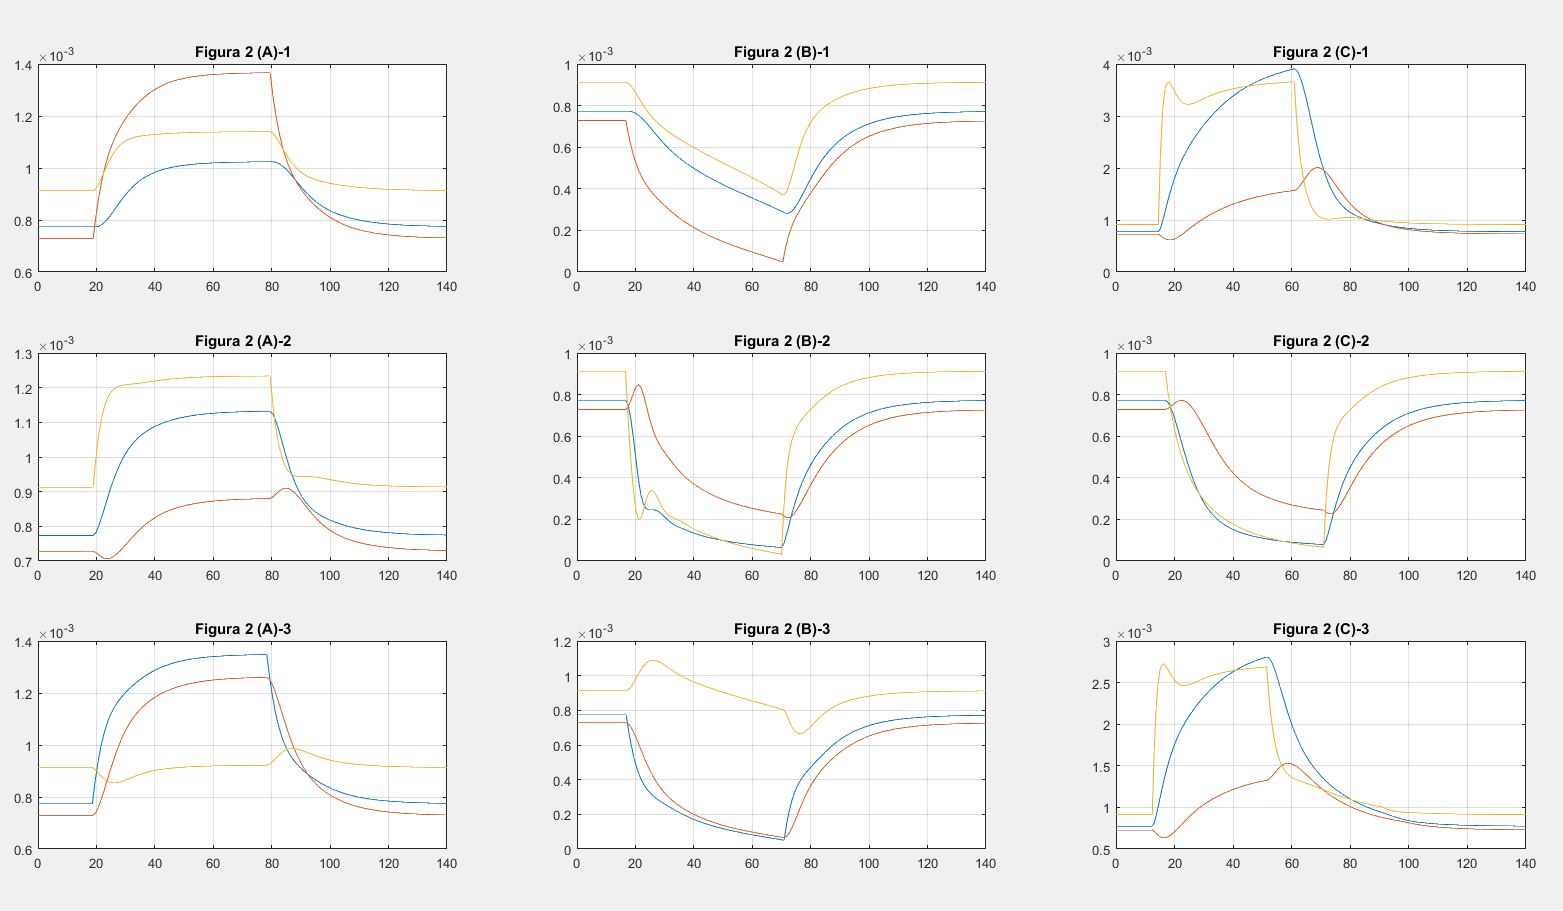
\includegraphics[width=0.99\textwidth]{GraficosLindos.JPG}
	\caption{Aproximaciones conseguidas mediante el algoritmo realizado.}
\end{figure}	


\section{Conclusión}
Comparando los gráficos obtenidos con los presentados en el artículo, se puede observar que las aproximaciones, realizadas con una tolerancia de $10^{-6}$, son buenas, es decir, próximas a las empleadas en el artículo. 	
 
\end{document}
